%!TEX root = emnlp2016.tex


% *** results ***
% (1) 1970s cables data; details
%     how we trimmed; how we selected the vocabulary
% (2) we fit the model; 100 topics
%     what we found
% (3) simulations
%     (a) how we simulated data; size, etc.
%     (b) competing methods
%     (c) results

% - divde into pghs
% - made f clear on our model
% - make comparison methods clear (citations)
% - make evaluation metrics clear (citation?)
% - how long does it take to fit the model
% - address simulate then fit
% - details on simuated data; do other methods scale?

% ========================

In this section we explore the performance of Capsule on a collection of U.S. State Department diplomatics cables and on simulated data.

\parhead{Data.}
The National Archive collects communications between the U.S. Sate department and its embassies.  We obtained a collection of these diplomatic messages from the History Lab at Columbia,\footnote{http://history-lab.org} which received them from the Central Foreign Policy Files at the National Archives.  The communications in this data set were sent between 1973 and 1978.

In addition to the text of the cables themselves, each document is supplemented with information about who sent the cable (e.g., the State Department, the U.S. Embassy in Saigon, or an individual by name), who received the cable (often multiple entities), and the date the cable was sent.  We used a vocabulary of size 6,293 and omitted cables with fewer than three terms, resulting in a collection of 2,139,324 messages sent between 27,134 entities.  We selected a weekly duration for the time intervals, as few cables were sent on the weekends.

\parhead{Model settings.}
We fit Capsule with $K=100$ general topics and using an exponential decay $f$,
\begin{equation}
f(i_d, t) = 
\begin{cases}
    0,			& \text{if } t > i_d\\
    \exp\{-(i_d - t) / \tau\},          & \text{otherwise,}
\end{cases}
\label{eq:f}
\end{equation}
with mean lifetime $\tau=3$.  This mean lifetime indicates that most intervals would no longer be relevant after about three weeks.  With these settings on the cables data, fitting the model takes 2.8 hours per iteration;\footnote{Our algorithm is batch--we consider each data point for every iteration.  Modifying the algorithm to stochastically sample the data would reduce the time required to achieve an equivalent model fit.} results are shown on 15 iterations.

\parhead{Results.}
We begin our exploration by detecting events using Capsule.  With \Cref{eq:eventness} as our metric of ``eventness,'' we consider this metric over time, which is shown in \Cref{fig:cables_events}.  Here, peaks correspond to real-worlds events, several of which are labeled.\footnote{Appendix~\ref{sec:additional_results} contains an analogous figure on arXiv data, which shows that Capsule does not capture weekly events on data that does not contain real-world events at that resolution.}

The tallest peak occurs the week of December 1, 1975, just prior to the Indonesian invasion of East Timor, which began December 7, 1975.  As discussed in \Cref{sec:model}, we sort documents by their event relevancy parameters $\epsilon$ to find cables that reflect an event.  \Cref{tab:timor} shows the top cables for the East Timor invasion.  Capsule accurately identifies this real-world event and recovers relevant cables.

\begin{table*}[tb]
\small
\centering
\begin{tabular}{cccl}
\toprule
$\epsilon$ & date & entity & subject \\
\midrule
0.124   &  1975-12-03  &  State  & President's talking point on Portuguese Timor \\
%0.121   &  1975-12-03  &  State  & President's talking point on Portuguese Timor \\
0.115   &  1975-12-04  &  State  & Timor we are repeating FYI a DAO message \\
0.112   &  1975-12-04  &  State  &  Legal problems relating to Portuguese Timor\\
0.105   &  1975-12-04  &  Secretary Peking & US Support for Timor resolution \\
0.102   &  1975-12-07  &  State  & Invasion of Portuguese Timor \\
\bottomrule
\end{tabular}
\label{tab:timor}
\caption{Top documents for the time interval of week December 1, 1975, just prior to the Indonesian invasion of East Timor, which began December 7, 1975; Capsule recovers relevant documents related to this real-world event.}
\end{table*}

\begin{table*}[htb]
\small
\centering
\begin{tabular}{cccl}
\toprule
$\epsilon$ & date & entity & subject \\
\midrule
0.090   &  1975-04-24  &  Mansfield, Mike & Assistance in evacuating family from South Vietnam \\
0.089   &  1975-04-24  &  Railsback, Tom & Assistance in evacuating friend from South Vietnam \\
%0.088   &  1975-04-24  &  Mansfield, Mike  & Assistance in evacuating family from South Vietnam \\
%0.086   &  1975-04-24  &  Williams, Harrison &  Assistance in evacuating family from South Vietnam \\
0.086   &  1975-04-24  &  Koch, Edward & Assistance in evacuating family from South Vietnam \\
0.086   &  1975-04-21  &  Schweiker, Richard & Support in evacuating family from Vietnam \\
%$\vdots$ & $\vdots$ & $\vdots$ & $\vdots$ \\
0.081   &  1975-04-25  &  Ketchum, William & Movement of South Vietnamese refugees to Guam \\
0.080   &  1975-04-21  &  Scott, Hugh & Whereabouts of missionaries in Vietnam \\
\bottomrule
\end{tabular}
\label{tab:saigon}
\caption{Top documents for the time interval of week April 21, 1975, just prior to the fall of Saigon on April 30, 1975; Capsule recovers relevant documents related to this real-world event.}
\end{table*}

The second tallest peak occurs the week of April 21, 1975, just prior to the fall of Saigon on April 30, 1975; \Cref{tab:saigon} shows the top cables for this event, which reflect the evacuation efforts that occurred during that week.  Unlike the East Timor event, where the most relevant communication exists at an administrative level, the evacuation of Saigon is best captured by individuals seeking help for family and friends.

Another event peaks occurs the week of July 2, 1973; the top three words under event its description $\pi$ are \emph{bicentennial}, \emph{hijack}, and \emph{mercenary}.  Top cables under event relevancy $\epsilon$ surround the bicentennial celebration of United States (July 4, 1973) and the Air France hijacking incident that began on June 27: Israeli operatives rescued hostages from this incident on July 4th.

Capsule also identifies events with smaller peaks, such as the death of Mao Tse-tung.  One of the top cables for this event is sent by Kissinger to all post with public affairs guidance: %the subject \emph{Death of Mao Tse Tung -- Public Affairs Guidance}:
\begin{shaded*} \tt{1.  Missions should avoid all speculation about the 
possible effects of the death of Chairman Mao on
US-PRC relationships as well as impact on internal
Chinese developments.}

\tt{2.  Official comments should be limited to the statements
of top level administration officials, texts of which
will follow by SEPTEL and wireless file.}
\end{shaded*}
\noindent In the other top cables for this event, embassies generally reported on press reactions and condolence or memorial ceremonies at their various locations.

Capsule helps discovers events which follow a chain of related incidents, though connecting these events is left to the investigator.  For example, Capsule discovers an event the week the Sinai Interim Agreement was signed (September 4, 1975), but it also detects an event in mid-October 1975 about the hiring of observers and technicians for the Sinai peace keeping force.  Associated with this second event is a cable from London to the State department entitled \emph{FCO views on Syrian stance}:
\begin{shaded*} \tt{Since conclusion of Sinai II negotiations, FCO
officials have expressed considerable interest in prospects
for next US effort to promote Syrian negotiations with Israelis. ...}
%Basic FCO position remains one of pervasion admiration for success of 
%Secretary's tactics with Egyptians and Israelis tempered by recognition that
%Syrian negotiating position will be a very tough nut to crack.  
%During recent ...}
\end{shaded*}
\noindent This cable and the sequence of events discovered by Capsule indicate that there is a longer lasting underlying situation.  Capsule cannot capture every aspect of these larger sequences of events, but it can provide insight into key moments so that investigators can explore both short-lived events and long-lasting political situations.

\begin{table}
\centering
\small
\begin{tabular}{c}
\toprule
top terms \\
\midrule
outlook, review, hire, personnel, invite, prepare \\
arrest, incident, security, family, guard, death, jail \\
locate, home, son, death, please, contact, father \\
request, refugee, response, service, sale, asylum \\
market, report, commercial, food, import, commerce \\
fear, leadership, back, arm, role, threaten \\
hotel, travel, reservation, visit, arrange, schedule \\
\bottomrule
\end{tabular}
\label{tab:topics}
\caption{Top vocabulary terms for a selection of general topics, one per row, according to topic distributions $\beta_k$.  Capsule identifies general diplomatic themes that can be relevant to any entity.}
\end{table}

\begin{table}
\centering
\small
\begin{tabular}{cc}
\toprule
entity & top terms \\
\midrule
State & request, follow, embassy, meet, make \\
Bangkok & bangkok, thailand, thai, refugee, follow \\
Jerusalem & jerusalem, israeli, bank, report, say \\
Stockholm & swedish, sweden, trade, meet, embassy \\
%Casablanca & casablanca, morocco, moroccan, request, please, note \\
Kampala & ugandan, nairobi, african, imperialist \\
Ndjamean & chadian, chad, lagos, drought, austerity \\
\bottomrule
\end{tabular}
\label{tab:entities}
\caption{Top vocabulary terms for a selection of entities according to entity-exclusive topics $\eta_n$.  Capsule identifies entity-specific themes and interests. }
\end{table}

In addition to events, Capsule can be used to explore the general themes of a corpus and entities' typical concerns.  Examples of general topics of conversation are shown in \Cref{tab:topics} and entity-exclusive topics are shown in \Cref{tab:entities}; these show us how entity topics absorb location-specific words, preventing these terms from overwhelming the general topics.

Appendix~\ref{sec:additional_results} contains additional examples of events discovered by Capsule, and more examples of general and entity-specific topics.

These exploratory results show that our model is successfully capturing when multiple entities are discussing the same subjects and that our model can be used to explore the underlying data by providing a structured scaffold from which to view the data.

\parhead{Simulations.}  We simulated data to provide a quantitative assessment of Capsule.
We generated twenty data sets, each with 100 time steps, 10 general topics, and 100 entities. Each simulation contained about 55,000 documents and followed the generative process assumed by Capsule, as shown in \Cref{fig:generative-model}.

\begin{figure}[t]
\centering
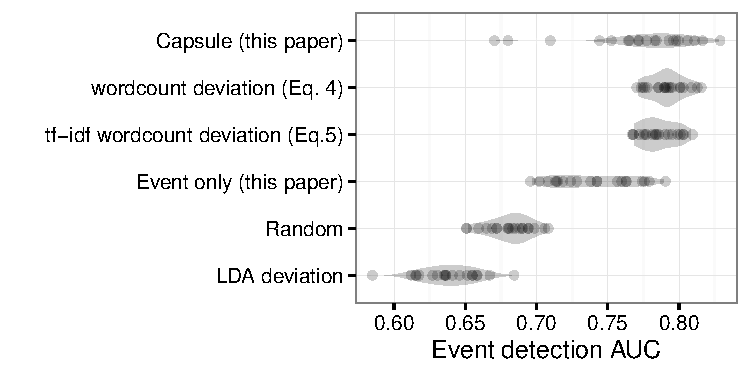
\includegraphics[width=\linewidth]{fig/sim_eventdetect.pdf}
\caption{Event detection performance on twenty simulated datasets.  Capsule is able to detect events as well as comparison methods, but its performance has higher variance.}
\label{fig:sim_eventdetect}
\end{figure}

To evaluate event detection, we created a ranked list of all time intervals and computed the overlap between a method and the simulated ground at every threshold; this generates an curve under which we cam compute the area and normalized based on ideal performance---we refer to this metric as event detection AUC. 

%^ XXX citation
 
The most successful of the baseline methods for event detection was average absolute error in word count relative to the mean, or
\begin{equation}
	\sum_{v=1}^V\left[\sum_{d=1}^D \mbox{abs}\left( w_{d,v} - \frac{1}{\vert D \vert}\sum_{d=1}^D w_{d,v} \right) \right],
\label{eq:wordev}
\end{equation}
and its tf-idf variant, 
\begin{equation}
	\sum_{v=1}^V\mbox{tf-idf}(v)\left[\sum_{d=1}^D \mbox{abs}\left( w_{d,v} - \frac{1}{\vert D \vert}\sum_{d=1}^D w_{d,v} \right) \right].
\label{eq:tfidfwordev}
\end{equation}
\Cref{fig:sim_eventdetect} shows that Capsule can outperform these approaches for event detection, but that it has higher variance in performance.  We also consider an ``event only'' model---this is a model that only uses the interval-related subset of Capsule's parameters; comparing to this shows that is it important to model ``business as usual'' for improved event detection.  LDA based approaches like average deviation from mean in topic space~\cite{dou2012leadline} do not perform well for event detection as deviations in topic space are too coarse to provide a meaningful signal.

\begin{figure}[h]
\centering
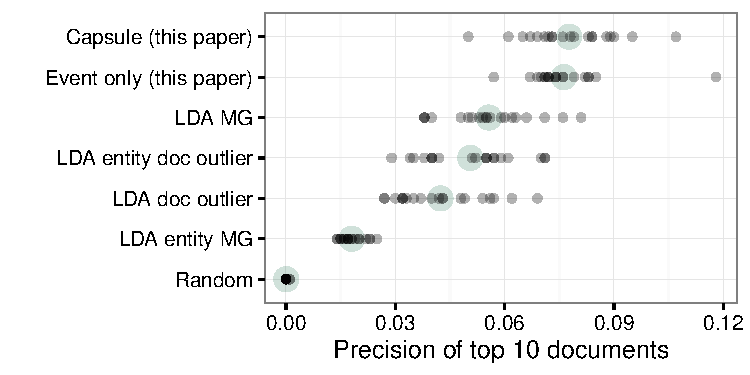
\includegraphics[width=\linewidth]{fig/precision10.pdf}
\caption{Precision of recovering the top ten most relevant documents, averaged over all time intervals.  Capsule performs best, averaged over twenty simulations.}
\label{fig:sim_precision}
\end{figure}

Once events have been identified, our next task is to identify relevant documents; to evaluate this, we calculate precision of recovering the top ten documents.  LDA is useful in finding relevant documents by selecting documents that deviate from the mean in topic space.  Word count deviations for each document (similar to Equations~\ref{eq:wordev} and~\ref{eq:tfidfwordev}) perform close to random for document recovery.

Finding documents based on absolute deviation from the mean works better in LDA topic space, but devnot over the full vocabulary.  Word count deviations, which performed well for event detection, performed worse than random for document recovery.  Both Capsule and its event-only partial model outperform all comparison methods in terms of document recovery.  \Cref{fig:sim_precision} shows precision of recovering the top ten documents.

We assessed the sensitivity of our model to three different decay functions $f$: exponential, linear, and step functions.  We simulated data for each function and then fit Capsule using every permutation of $f$ and multiple settings for event decay duration.  In all cases, we found that the model is not sensitive to decay shape or duration; details are in Appendix~\ref{sec:additional_results}.

\parhead{Comparisons on Cables.}
We ran the word count based approaches on the cables data and found that they were difficult to interpret and did not recover important historical events.  For instance, none detected the evacuation of Saigon, a major historical event in the corpus.  The LDA-based approaches do not yield large gains in run time over Capsule and do not provide the granularity needed to capture substantial events.